%\documentclass[twocolumn]{article}
\documentclass{article}

%\usepackage{arxiv}

\usepackage[backend=biber, style=numeric]{biblatex} % Use Biber and APA style

\addbibresource{references.bib} % Load your .bib file

\usepackage[utf8]{inputenc} % allow utf-8 input
\usepackage[T1]{fontenc}    % use 8-bit T1 fonts
\usepackage{hyperref}       % hyperlinks
\usepackage{url}            % simple URL typesetting
\usepackage{booktabs}       % professional-quality tables
\usepackage{amsfonts}       % blackboard math symbols
%\usepackage{nicefrac}       % compact symbols for 1/2, etc.
%\usepackage{microtype}      % microtypography
\usepackage{lipsum}		% Can be removed after putting your text content
\usepackage{graphicx}
%\usepackage{natbib}
\usepackage{doi}
\usepackage{amsmath}
\usepackage{amsfonts}
\usepackage{bbm}

%\usepackage{biblatex}

\usepackage{grffile}
\usepackage{authblk}

\usepackage[switch,columnwise]{lineno}
\linenumbers
\usepackage{fixmetodonotes}
\usepackage{multirow} % Needed for merging cells vertically
\usepackage{makecell} % For multi-line cells
\usepackage{booktabs} % For nicer table lines
\usepackage{adjustbox} % For table adjustments

% Import bibliography
%\bibliography{anoruti_refs.bib}
%\addbibresource{anoruti_refs.bib}


%opening
\title{Modeling the dynamics of bacterial colonisation in a murine model of Urinary Tract Infections}
\author[1]{Carlos Olivares}
\author[1]{Charles Burdet}
\author[1]{Ariane Amoura}
\author[1]{Imane El Meouche}
\author[1,2]{Emmanuelle Comets}

\affil[1]{Universit\'e Paris Cit\'e and Universit\'e Sorbonne Paris Nord, Inserm, IAME, F-75018 Paris, France}
\affil[2]{Univ Rennes, Inserm, EHESP, Irset - UMRS 1085, 35000 Rennes, France}
%\institute[shortinst]{\inst{1} \textit{Universit\'e Paris Cit\'e and Universit\'e Sorbonne Paris Nord, Inserm, IAME, F-75018 Paris, France} \samelineand \inst{2} \textit{Univ Rennes, Inserm, EHESP, Irset - UMRS 1085, 35000 Rennes, France}}


\begin{document}

\maketitle

\begin{abstract}
	
\TODO{Change Abstract}
%Ariane's paper summary:

%Urinary tract infection (UTI), mainly caused by Escherichia coli, are frequent and have a recurrent nature even
%after antibiotic treatment. Potential bacterial escape mechanisms include growth defects, but probing bacterial division in vivo and establishing its relation to the antibiotic response remain challenging. Using a synthetic reporter of cell division, we follow the temporal dynamics of cell division for different E. coli clinical
%strains in a UTI mouse model with and without antibiotics. We show that more bacteria are actively dividing in the kidneys and urine compared with the bladder. Bacteria that survive antibiotic treatment are consistently non-dividing in three sites of infection. 
%Additionally, we demonstrate how both the strain in vitro persistence profile and the microenvironment impact infection and treatment dynamics. Understanding the relative
%contribution of the host environment, growth heterogeneity, non-dividing bacteria, and antibiotic persistence is crucial to improve therapies for recurrent infections.
\end{abstract}

\section{Introduction}



\begin{itemize}
	\item Importance, motivation Why?
	\item What is know about it?
	\item What is the purpose of this work?
	\item Migration dynamics depends on the bacteria strain.
	\item Urinary tract infections (UTI) are the second most common infection worldwide with high recurrence rates, with E. coli the most prevalent cause of infection \cite{rosen2007detection}.
	\item Understanding the survival mechanisms and prevalence of these pathogens plays an important role in avoiding resistant bacteria's appearance and proliferation and tolerance.
	\item How to explain that non-dividing bacteria are the ones that survives?
\end{itemize}

\section{Methods}






\subsection{Data Description}

%\begin{itemize}
%	\item  the second paragraph is out of order, start with the sampling protocol, how
%	organs were recovered and weighted, and urine collection. Then how CFU were
%	obtained from these samples. "For urine..." (urine volume) you can keep it here
%	but you have to explain how that relates to CFU counts (it's not clear what the
%	units are).
%	the last sentence of this paragraph isn't grammatically sound so hard to understand.
%\end{itemize}

%draw_Anoruti_flowchart_PAS


A total of 203 healthy 8-week-old female CBA/J mice,  in an ascending pyelonephritis UTI mouse model \cite{labat2005mutator}, were bacteria infection were administered into the bladder through a urethral catheter after general anesthesia on day 0 with approximately $10^8$ colony-forming units (CFU) of PAS, NILS69, UTI, or CFT bacterial strains without any antibiotic treatment. Of these, 29 mice received ciprofloxacin at doses of either 2.5 mg/kg or 10 mg/kg over a 48-hour period.

The bacterial density (CFU/g or CFU/ml) in each organ was determined, after sacrifice by culturing the bacteria overnight in Luria-Bertani (LB) broth. Additional details can be found in \cite{amoura2024variability}.
CFU counts in each organ were calculated by scaling the CFU/g values obtained from the kidney and bladder based on the measurement of organ's weight after sacrifice. For urine we assumed a standard volume of 1 ml as a scaling factor. Mice without antibiotic treatment were sacrificed on days 1, 2, 4, 6, 10, 16, and 22, while those receiving antibiotic treatment were sacrificed on day 4 only. For more detailed information table, please refer  to Table \ref{tab:mice_sampling} in the supplementary materials.


%strain\cite{kotula2014programmable},  and divided in three groups\cite{amoura2024variability}(76 mice without antibiotic, 17 with 2.5mg/kg and 7 with 10 mg/kg of ciprofloxacin during 2 days of treatment two times a day).








\subsection{Statistical model}

Nonlinear mixed effects modeling approach was used to analyze the different observations over time. A nonlinear mixed effects model for multiple responses is defined as follows. Let $y_i \equiv (y_{i,K}; y_{i,B}; y_{i,U})$ denote the vector of the number of CFU for kidney $y_{i,K}$, bladder $y_{i,B}$, and urine $y_{i,U}$ at time $t_i$ for individual $i$.
Let $f$ denote the global structural model characterizing all responses, based on a system of ordinary differential equations, similar for all individuals.
Then one can define $ y_{i,l} = f_{l}(\theta_i, \xi_{i,l} ) + \epsilon_{i,l} $ where $f_{l}$ is the component of the global model $f$ describing the $l$th response ($l \in \{K,B,U\}$), $\theta_i$ is the vector of individual parameters, $\xi_{i,l}$ is the vector of the $n_{i,l}$ sampling times and $\epsilon_{i,l}$ is the vector of residual errors for the  response $l$ in individual $i$. Each individual parameter $\theta_i$ can be decomposed as a fixed effect $\mu$, which represents the mean value of the parameter in the population, and a random effect $b_i \sim \mathcal{N}(0, \Omega)$ where $\Omega$ accounts for the inter-individual variability. Assuming an exponential random effect model, the individual parameters are modeled as : $\theta_i = \mu \exp(b)$.
Lastly we assumed that $\epsilon_{i,l} \sim \mathcal{N} (0, \Sigma_{i,l})$ where $\Sigma_{i,l}$ is a $ n_{i,l} \times n_{i,l}$-diagonal matrix with $l$th elements equal to $(\sigma_{inter,l} + \sigma_{slope,l}\times f_{l}(\theta_i, \xi_{i,l}))^2$ with $\sigma_{inter, l}$ being the paremeter for the additive part and $\sigma_{slope,l}$ the parameter for the proportional part of the variance error model. Constant ($\sigma_{inter, l} \neq 0$, $\sigma_{slope, l} = 0$), proportional ($\sigma_{inter, q} = 0$, $\sigma_{inter, l} \neq 0$, ) or combined ($\sigma_{inter, l} \neq 0$, $\sigma_{slope, l} \neq 0$ ) variance error models were tested for each response $l$.





\subsection{Modeling Strategy}


\subsubsection{Modeling PAS strain}

To investigate bacterial dynamics in a mouse model of urinary tract infection, we tested two structural models: a logistic growth model \cite{allen2018bacterial}, shown in Eq. (\ref{eq:ODElogistic}), and an effective net rate model in Eq. (\ref{eq:ODEeffect}). Evaluating both models across each of the three defined compartments: kidney ($K$), bladder ($B$), and urine ($U$). The logistic growth model combines linear growth with a non-linear elimination rate, for saturation effects. In contrast, the net rate model considers the overall linear growth and elimination effects, simplifying the dynamics by focusing on net changes of proliferation and elimination in each compartment.

The logistic growth model for a compartment $X$ is defined as


\begin{alignat}{2}
\frac{d}{dt} N_{X} &=  \alpha_X \left( 1 - \frac{ N_{X} }{ N_{X}^{ss} }\right)N_{X}  & + \sum_{Y \neq X}^{\mathcal{O} } \left( -q_{X,Y} N_{X} + q_{Y, X} N_{Y} \right)
\label{eq:ODElogistic}
\end{alignat}



%\begin{alignat}{2}
%\frac{d}{dt} K &=  \alpha_K \left( 1 - \frac{K}{K^{ss}}\right) K & -q_{K,B} K + q_{B,K} B \nonumber \\
%&              & -q_{K,U} K + q_{U,K} U \nonumber \\
%\frac{d}{dt} B &=  \alpha_B \left( 1 - \frac{B}{B^{ss}}\right) B & -q_{B,K} B + q_{K,B} K  \nonumber \\
%&              & -q_{B,U} B + q_{U,B} U \nonumber \\
%\frac{d}{dt} U &= \alpha_U \left( 1 - \frac{U}{U^{ss}}\right) U &- q_{U,B} U + q_{B,U} B \nonumber \\
%&              & -q_{U,K} U + q_{K,U} K\nonumber \\
%\label{eq:ODElogistic}
%\end{alignat}
% I should defined as cause, effect instead of from X to Y, that was pretty dumb.
where $N_{X}$ is the amount of CFU in compartment $X$, $\mathcal{O} \equiv \{K,B,U\}$ is the set of all compartments, $\alpha_{X}$ the bacterial growth rate, $N^{ss}_{X}$ the carrying capacity which defines the saturation point of bacteria in each compartment, and $q_{X,Y}$ the migration or exchange rates from compartment $X$ to compartment $Y$ where $X,Y \in \mathcal{O}$.

The net rate model,  for all compartments is defined as

%\TODO{Net rate of change}


\begin{alignat}{2}
\frac{d}{dt} N_{X} &=  \delta_X N_{X} & + \sum_{Y \neq X}^{\mathcal{O} } \left( -q_{X,Y} N_{X} + q_{Y, X} N_{Y} \right)
\label{eq:ODEeffect}
\end{alignat}



%\begin{alignat}{2}
%\frac{d}{dt} K &=  \delta_K K &- q_{K,B} K + q_{B,K} B \nonumber \\
%&              & -q_{K,U} K + q_{U,K} U \nonumber \\
%\frac{d}{dt} B &=  \delta_B B &- q_{B,K} B + q_{K,B} K \nonumber \\
%&              & -q_{B,U} B + q_{U,B} U \nonumber \\
%\frac{d}{dt} U &= \delta_U U &- q_{U,B} U + q_{B,U} B \nonumber \\
%&              & -q_{U,K} U + q_{K,U} K \label{eq:ODEeffect}
%\end{alignat}


where $\delta_X$ is the effective net rates(proliferation if positive and elimination if negative) which is the overall result of both linear proliferation and elimination rates that cannot be distinguished from the data.


%\begin{alignat}{2}
%\frac{d}{dt} K &=  \rho_K K &- q_{K,B} K + q_{B,K} B \nonumber \\
%&              & -q_{K,U} K + q_{U,K} U \nonumber \\
%\frac{d}{dt} B &=  \rho_B B &- q_{B,K} B + q_{K,B} K \nonumber \\
%&              & -q_{B,U} B + q_{U,B} U \nonumber \\
%\frac{d}{dt} U &= \rho_U U &- q_{U,B} U + q_{B,U} B \nonumber \\
%&              & -q_{U,K} U + q_{K,U} K \label{eq:ODEeffect}
%\end{alignat}


We studied the natural progression of infection and bacterial spread without external intervention considering only mice without antibiotic treatment and infected with PAS strain. We selected the optimal structural model by testing all possible combinations of logistic growth and net rate models across the compartments (kidney, bladder, urine), without accounting for inter-individual variability. For example, one combination could involve logistic growth in the kidney while applying net rate models to the bladder and urine. This allowed us to determine which structural combination best describes bacterial dynamics across the different compartments.
%
After selecting the optimal structural model, we evaluated exchange rates between compartments to further simplify the model. We then introduced inter-individual variability sequentially to each parameter, repeating this process until no further model improvement was observed.


\subsubsection{Modeling strain effect}

Finally, to investigate strain-specific differences in the dynamics, we used the PAS strain as a reference and employed a forward covariate selection procedure on all model parameters one at the time until no model improvement.


%Finally, we studied strain difference in the dynamics starting with the PAS strain as reference and using a forward covariate selection procedure on all parameters model. 


%Starting with the PAS strain as the base model, additional bacterial strains were tested individually as covariates. The Bayesian Information Criterion corrected for small sample sizes (BICc) was used to assess model improvement, with strains retained if they led to a reduction in BICc.


%\begin{alignat}{2}
%\frac{d}{dt} X &=  \alpha_X \left(1 - \frac{X}{X^{ss}} \right) X + \sum_{Y \neq X} \left( - q_{X,Y} X + q_{Y,X} Y \right) & \text{Logistic Growth} \label{eq:ODElogistic} \\
%\frac{d}{dt} X &=  \delta_X X + \sum_{Y \neq X} \left( - q_{X,Y} X + q_{Y,X} Y \right) & \text{Effective elimination/proliferation}
%\label{eq:ODEeffect}
%\end{alignat}



%\begin{equation}
%\frac{d}{dt} X =  \alpha_X \left(1 - \frac{X}{X^{ss}} \right) X + \sum_{Y \neq X} \left( - q_{X,Y} X + q_{Y,X} Y \right)
%\end{equation}


%\begin{equation}
%	\frac{d}{dt} X =  \delta_X X + \sum_{Y \neq X} \left( - q_{X,Y} X + q_{Y,X} Y \right)
%\end{equation}





\subsubsection{Modeling PAS strain under antibiotic treatment}

%Due to the lack of antibiotic concentration measurements we modeled the effect of the antibiotic in the net rate only $\delta_{X}$, where $X \in \{K,B,U\}$, assuming that there is no direct effect on the compartment exchange rate.

In the absence of antibiotic concentration data, we modeled the antibiotic's effect assuming no direct influence of the antibiotic on the exchange rates between compartments and solely through its impact on the net bacterial growth rates ($\delta_{X}$, where $X \in \{K,B,U\}$ for the kidney, bladder, and urine compartments). 

The net rate under an antibiotic administration is given by: 
\begin{equation}
\delta_{X}^{Ab} = \left( 1 + \mathcal{A}_{X}(D^{Ab}) \right) \delta_{X}
\label{eq:deltaAntibiotic}
\end{equation}
%As shown in Eq. \ref{eq:deltaAntibiotic} the net rate is modified by an additive factor $\mathcal{A}(D^{AB} )$ 
%Eq. \ref{eq:deltaAntibiotic} 
where $\mathcal{A}_{X}(D^{Ab})$ is the functional dependency of corresponding administrated dosage $D^{AB}$, and $\delta_X$ denotes the net rate in compartment $X$ without the antibiotic effect, where $X \in \{K, B, U\}$.

We evaluated three different structural forms of the antibiotic effect: no effect Eq. (\ref{eq:modelABNoEffect}), a linear effect Eq. (\ref{eq:modelABLinear}), and a non-linear effect Eq. (\ref{eq:modelABNonLinear}) that is not proportional to dosage

\begin{alignat}{2}
	\mathcal{A}_{X}(D^{Ab}) &= 0, &\quad\quad\quad \text{no effect} \label{eq:modelABNoEffect} \\
	\mathcal{A}_{X}(D^{Ab}) &= \epsilon_{X} D^{Ab}, &\quad\quad\quad \text{linear} \label{eq:modelABLinear}\\
	\mathcal{A}_{X}(D^{Ab}) &= \mathbb{I}_{D^{Ab},D_1} \Phi_{D_1}^{X} + \mathbb{I}_{D^{Ab},D_2} \Phi_{D_2}^{X}, &\quad\quad\quad \text{non-linear} \label{eq:modelABNonLinear} 
\end{alignat}
where $\epsilon_{X}$  is the constant rate of the impact of the antibiotic, $D_l$ is the dosage $l$ ($l=1,2$ for dosage 1 and 2) of the antibiotic $Ab$, $\mathbb{I}_{D^{Ab},D_l}$ is 1 if $D^{Ab} = D_l$ and 0 otherwise, $\Phi_{D_l}^{X}$ is the parameter that characterize the effect of the dosage $l$ in compartment $X$.

Given the limited data available for mice with antibiotic treatment, we investigated the influence of antibiotics on the PAS strain by maintaining the model parameters unchanged from the non-antibiotic scenario. To assess the antibiotic effect, we explored various possibilities: no effect Eq. (\ref{eq:modelABNoEffect}), linear Eq. (\ref{eq:modelABLinear}) and nonlinear Eq. (\ref{eq:modelABNonLinear}) dependencies on dosage across all compartments. Once the optimal model capturing the antibiotic effect was identified, we simplified the model by examining the impact of antibiotics on each compartment individually.


Based on PAS model, we studied the antibiotic effects for the mice treated with two different ciprofloxacin doses $D_1 = 2.5 mg/kg $ and $D_2 = 10 mg/kg$ by fixing the parameters of the model without antibiotic and selected the best model considering all possible combinations of the effect in each compartment.

%Modeling_ms_03_AB_FIX_RespC.html

%%%%%%%%%%%%%%%%%%%%%%%%%%%



 Given the absence of measured drug concentrations, we assumed that the antibiotic primarily influences the effective growth rates of the bacteria. To explore this assumption, we tested three different models: a model with no effect of the antibiotic, a linear model with dose dependence, and a non-linear model to evaluate the impact of the antibiotic on bacterial dynamics.



%
%This process was repeated iteratively, with one covariate added at a time. The final model included only those covariates that significantly reduced BICc.


%\begin{alignat}
%	\frac{d}{dt} X = \alpha_{X} \left( 1 - \frac{X}{X^{ss}} \right)X + \sum_{Y \neq X} q_{X,Y} X + q_{Y,X} Y
%\end{alignat}


%\subsection{Parameter estimation}

\subsection{Model selection and evaluation}

Estimation of population parameters was performed using the stochastic approximation expectation maximization algorithm (SAEM) \cite{kuhn2005maximum}, implemented in Monolix 2021R2 (Lixoft, Orsay, France, www.lixoft.eu), a software devoted to parameter estimation by maximum likelihood in nonlinear mixed effect models. Data below the lower limit of quantification were treated as left-censored data. Their contribution to the likelihood was computed as the probability that these data are indeed below the lower limit of quantification\cite{samson2006extension}. 

Model selection was guided by comparing BICc with threshold of 2 points difference and improvement of parameters uncertainty with $RSE < 100\%$. The final model was selected based on the best fit to the data. 
%\TODO{detail model strategy in accordance with new figure 2 to 3.}

Model evaluation was carried out using several goodness-of-fit plots, particularly individual fits, normalized prediction distribution errors (NPDEs) vs. time and NPDE vs. predictions, and visual predictive checks (VPCs) generated with monolix.


\subsection{Simulations}
%\TODO{Detail simulations}
%\begin{itemize}
%	\item Simulations for PAS, and strains, done with simulx, etc
%	\item Number of virtual mice?
%	\item Definition of time to clearance?
%	\item What else could we explore in simulations?
%\end{itemize}


We performed computational simulations to study bacterial infection dynamics and clearance in a population of 1,000 virtual mice, both with and without antibiotic treatment. These simulations were carried out using Simulx 2021R2 and modeled bacterial growth, migration between organs, and the effects of antibiotics.

To account for individual variability, parameter values for bacterial growth, elimination rates, and migration were drawn from corresponding distributions. Additionally, covariates for different bacterial strains were included to evaluate the impact of strain-specific characteristics on infection outcomes. Bacterial clearance probabilities were calculated at each time step throughout the simulation.

In the model, infection was considered cleared in each organ when 95\% of the virtual mice had bacterial levels below 1 CFU in that organ.





\section{Results}

\subsection{Data}


Of the total of 203 healthy 8-week-old female CBA/J mice 179 were divided in four groups with the 76(PAS), 27(NILS69), 31(UTI), 40(CFT) (see Table \ref{tab:mice_sampling}) were analyzed in three groups: First, only mouse with no antibiotic treatment and infected with PAS strain to determine the natural progression of the infection. 

%\begin{itemize}
%	\item How mice data was collected, sacrifice, catheter, etc.
%	\item Describe the organ med [min, max] weight
%	\item med [min, max] CFU per day and organ.
%	\item Specified the dosage of ciprofloxacin and 48 hours duration, with a twice a day administration.
%	\item Make reference to figure with fits shown next section, for both strains (covariates) and antibiotic effect.
%	\item Maybe LacZ fraction. Probably not
%\end{itemize} 

\subsection{Model Selection}

\begin{figure}
	\centering
	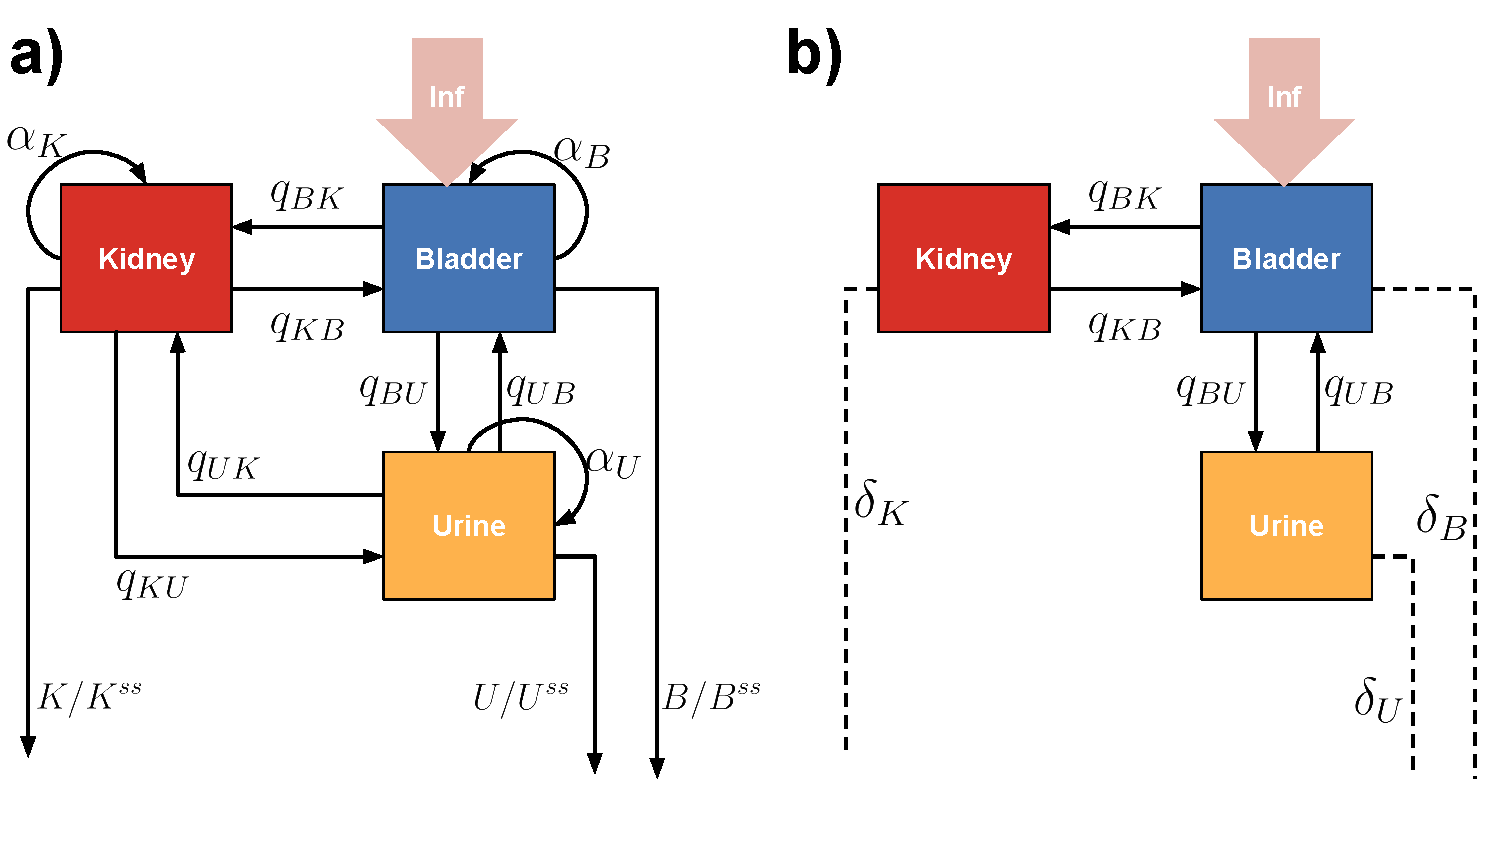
\includegraphics[width=0.8\linewidth]{images/draw_Anoruti_Models_schema.pdf}
	%	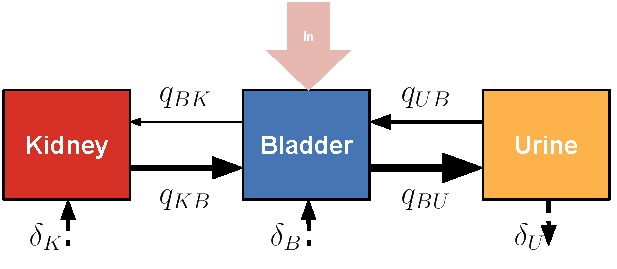
\includegraphics[width=0.4\linewidth]{images/draw_Anoruti_Compartments_oneline_v001.pdf}
	\caption{a) Logistic growth initial model b) net rate of change final model without antibiotic treatment. }
	\label{fig:ModelOnelineNOATB}
\end{figure}


To characterize the dynamics of bacterial infection in kidney, bladder, and urine compartments in untreated mice, we evaluated logistic growth and net rate models across each compartment. A series of candidate models with various combinations of logistic growth and net rate dynamics were compared using Bayesian Information Criterion (BIC) values, as shown in Table \ref{tab:ModelSelectionPASLogvsNet}.



%688.156 NOSS qUs



%\begin{itemize}
%	\item Make summary table with the BICs of the models without variability to shown the improvement of model selection.
%	\item Do the same for model with strains and antibiotic, but probably in supplementary information.
%\end{itemize}

\subsection{Final Models and Estimated Parameters}

Here we describe the final models and their respective estimated parameters for analyzed case


\subsubsection{Model for PAS strain}

For the group with PAS only the model was best described by net rates model with 
migration exchanges on bladder to kidney, kidney and urine as show in figure \ref{fig:ModelOnelineNOATB}b, details on BICc selection performance are provided in supplemetary material.


\begin{table}
	\begin{tabular}{|l|l|l|l|}
		\hline
		Logistic model & Net rate model & BICc & Model nickname\\ \hline
		$K, B, U$ &           & 803.117 & General \\
		$K, B   $ & $U   $ & 709.026 & NOSS U \\
		$B, U   $ & $K      $ & 717.472 & NOSS R \\
		$K, U   $ & $B      $ & 709.307 & NOSS V \\
		$K      $ & $B, U   $ & 713.777 & NOSS VU \\
		$U      $ & $K, B   $ & 714.093 & NOSS RV \\
		$B      $ & $K, U   $ & 714.535 & NOSS RU \\
		& $K, B, U$ & 702.108 & NOSS RVU \\
		$       $ & $K, B, U$ wo UR & \textbf{688.156} & NOSS RVU without exchanges between U and R \\
		%		          & $K, B, U$, without $q_{K,U}$ and $q_{U,K}$ & \textbf{688.156} & \textbf{NOSS qUs} \\
		\hline
	\end{tabular}
	\label{tab:ModelSelectionPASLogvsNet}
	\caption{Model selection process for a structural model, where logistic and net rate models are applied to different compartments. The Logistic model and Net rate model columns indicate which model is used in each compartment. The BICc column shows the Bayesian Information Criterion. }
\end{table}


\begin{itemize}
	\item \TODO{Add monolix structural model in appendix}
	\item \TODO{Think in a way to encapsulate all the BICc for each model in a single table with the covariates BICc, and maybe move it to supp.}
\end{itemize}

Final selected model defined by Eq. (\ref{eq:FinalModelPASK}-\ref{eq:FinalModelPASU}) is composed using only net rate model for all compartments, represented in Fig. \ref{fig:ModelOnelineNOATB}b, and with estimated parameter in table \ref{tab:FinalModelPAS}.

\begin{alignat}{2}
\frac{d}{dt} K &=  \delta_K K &- q_{K,B} K + q_{B,K} B \label{eq:FinalModelPASK} \\
\frac{d}{dt} B &=  \delta_B B &- q_{B,K} B + q_{K,B} K \nonumber\\
&              & -q_{B,U} B + q_{U,B} U \label{eq:FinalModelPASB} \\
\frac{d}{dt} U &= - \delta_U U &- q_{U,B} U + q_{B,U} B \label{eq:FinalModelPASU}
\end{alignat}
%\end{equation}


The estimated parameters for the model for strain PAS. without antibiotic treatment capture the rates of bacterial net proliferation or clearance and transfer between different compartments, as well as associated variabilities. Specifically, $\delta_{K}$ and $\delta_{B}$ represent a similar net proliferation in kidney and bladder around $12$ CFU/day. Meanwhile, in the urine compartment a net elimination represented in $\delta_{U}=9.75$ CFU/day.

The parameters $q_{BK}=0.0021$ CFU/day describe a slow bacteria transfer from bladder to kidney been the parameter with highest uncertainty(92.3\%) which contrast with the high bacteria transfer from kidney to bladder $q_{KB} = 12.3$ CFU/day that has been precise estimated (1.06\%). This suggest that as infection start in bladder, even with a slow migration rate the high proliferation rate rapidly increase the amount of bacteria in kidney. Now the fast migration rate from kidney to bladder $q_{KB}$ and from bladder to urine $q_{BU}=59.2$ CFU/day indicates that the effective elimination path is the done in urine.




\begin{table}
	\begin{tabular}{|l|l|l|l|}
		\hline
		Parameter & Estimates(r.s.e.) & Units\\ \hline
		$\delta_{K}$ & $12.2(1.09\%)$ & $(days)^{-1}$\\
		$\delta_{B}$ & $12.7(11.2\%)$ & $(days)^{-1}$\\
		$\delta_{U}$ & $9.75(30.6\%)$ & $(days)^{-1}$\\
		$q_{BK}$ & $0.0021(92.3\%)$ & $(days)^{-1}$\\
		$q_{KB}$ & $12.3(1.06\%)$ & $(days)^{-1}$\\
		$q_{BU}$ & $59.2(35.5\%)$ & $(days)^{-1}$\\
		$q_{UB}$ & $4.24(16.6\%)$ & $(days)^{-1}$\\
		$\omega_{\delta_{U}}$ & $3.36(36.9\%)$ & $(days)^{-1}$\\
		$\omega_{q_{BU}}$ & $0.231(25.3\%)$ & $(days)^{-1}$\\
		\hline
	\end{tabular}
\label{tab:FinalModelPAS}
	\caption{Estimates of model without antibiotic treatment for PAS straind, with variabilities in $\delta_U$ and $q_{BU}$ with normal and log-normal distribution respectively.}
\end{table}



\subsubsection{Model with different strains without antibiotic}

Here we present the model considering the four different strains in Table \ref{tab:FinalModelALLStrains}, as a main difference with the case with only PAS here we have the same elimination path in urine compartment. The proliferation rate in kidney gain a substantial increase, that is compensated by the substantial increase in transfer rate from kidney to bladder, as shown in Table \ref{tab:FinalModelALLStrains} and \ref{tab:FinalModelPAS}. At the main effect for CFT and UTI is slower elimination rate in urine and a faster elimination in urine for NILS69. However, we should notice that NILS69 is the strain with data only at days 2 and 4. Also notice that we get a reduction in the relative stantard error (r.s.e.) for the migration from bladder to kidney $q_{BK}$

\begin{table}
	\begin{tabular}{|l|l|l|l|}
		\hline
		Parameter & Estimates(r.s.e.) & Units\\ \hline
		$\delta_{K}$ & $40(0.74\%)$ & $(days)^{-1}$\\
		$\delta_{B}$ & $13(19.26\%)$ & $(days)^{-1}$\\
		$\delta_{U}$ & $12(33.15\%)$ & $(days)^{-1}$\\
		$q_{BK}$ & $ 0.0016(34.95\%)$ & $(days)^{-1}$\\
		$q_{KB}$ & $40(0.74\%)$ & $(days)^{-1}$\\
		$q_{BU}$ & $66(10.84\%)$ & $(days)^{-1}$\\
		$q_{UB}$ & $2(6.86\%)$ & $(days)^{-1}$\\
		$\omega_{\delta_{U}}$ & $1.2(15.28\%)$ & $(days)^{-1}$\\
		$\omega_{q_{BU}}$ & $0.11(40.13\%)$ & $(days)^{-1}$\\
		$\beta_{\delta_{U}, CFT}$ & $-1.1 (30.03\%)$ & $(days)^{-1}$\\
		$\beta_{\delta_{U}, UTI}$ & $-1.6 (23.54\%)$ & $(days)^{-1}$\\
		$\beta_{\delta_{U}, NILS69}$ & $3.8 (25.51\%)$ & $(days)^{-1}$\\
		%		$\sigma$
		\hline
	\end{tabular}
	\label{tab:FinalModelALLStrains}
	\caption{Estimates of the model parameters without antibiotic treatment for strains:PAS, CFT, UTI, NILS69, showing variabilities in $\delta_U$ and $q_{BU}$ with normal and log-normal distributions, respectively. $\beta_{\delta_U}$ represents the covariate effect on $\delta_U$ for each strain, with PAS as the reference strain.}
\end{table}


%plt_Ct_strain_ALL_covar_deltaU.pdf
\begin{figure}
	\centering
	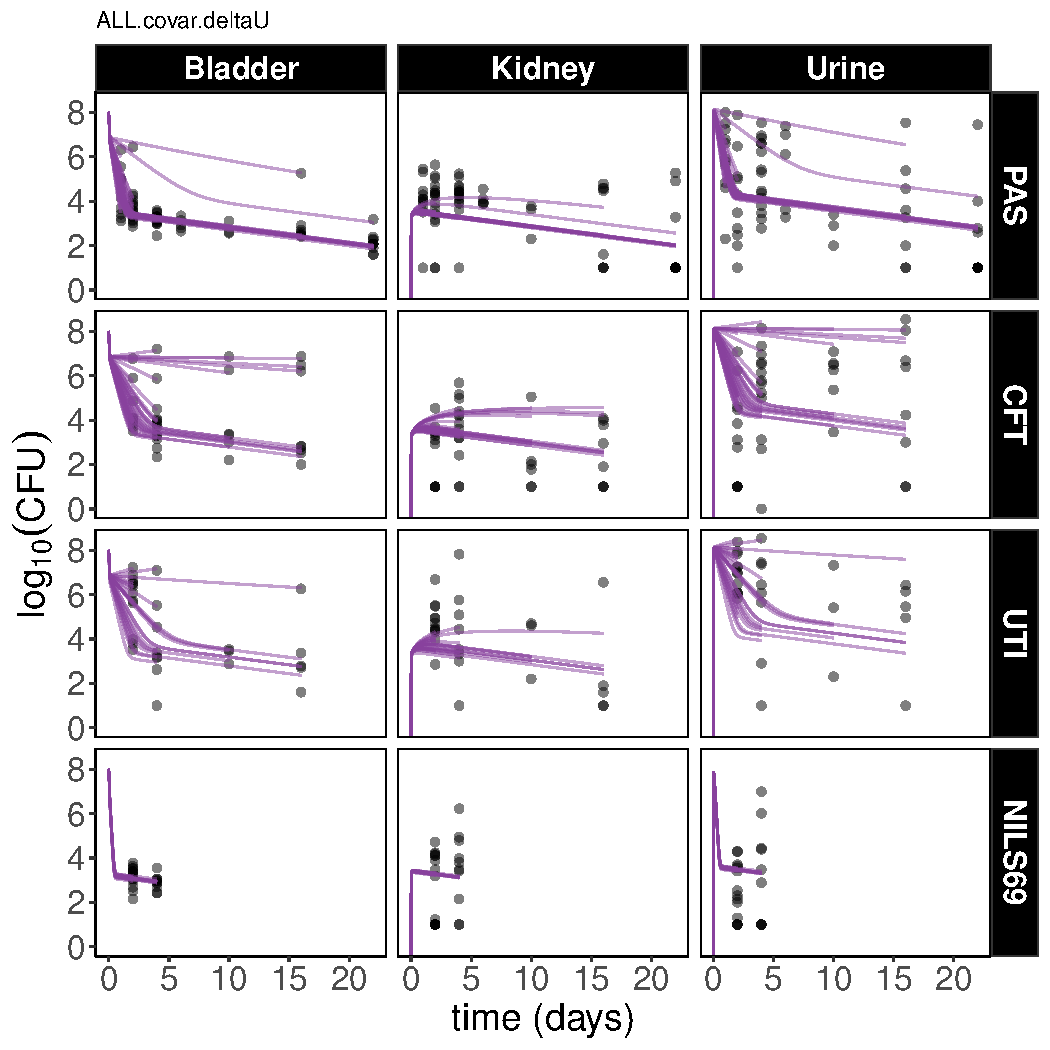
\includegraphics[width=\linewidth]{images/plt_Ct_strain_ALL_covar_deltaU.pdf}
	\caption{Time evolution of CFU for each organ compartment, open circles experimental data, individual fits gray line, purple curve population parameters for different strains.}
	%	, black solid line medianvalue at each sampling day
	\label{fig:ModelStrainsIndFits}
\end{figure}


\subsection{Simulations strains without antibiotic treatment}

We performed 1000 individual simulations, sampled from the model, for the different bacteria strains considering to evaluate the clearance different for the different strains.
We defined that a mouse cleared the bacteria if the CFU are bellow 1 and the time to clearance when at least 80\% of the sampled individuals reach the limit of 1 CFU, and the results of this- are shown in Fig. \ref{fig:SimulationsClearedStrainsALL}.

For the kidney compartment, strain NILS69 clears the fastest at 34.5 days, while UTI takes the longest at 55.5 days, indicating strain-dependent differences in clearance efficiency. Similarly, in the bladder, NILS69 again shows the shortest clearance time at 33.5 days, while UTI exhibits the longest time at 72.5 days, suggesting that UTI may be more resilient to clearance in this compartment.

In the urine compartment, NILS69 clears markedly faster than the other strains, achieving clearance in just 26 days. In contrast, UTI requires 94 days for clearance, underscoring a substantial difference in clearance rates for this strain compared to others. These results highlight NILS69 as the strain with the most rapid clearance across all compartments, while UTI consistently shows the slowest clearance, particularly in the bladder and urine. The findings suggest both compartment-specific and strain-specific factors influence the time required for bacterial clearance.



\begin{figure}
	\centering
	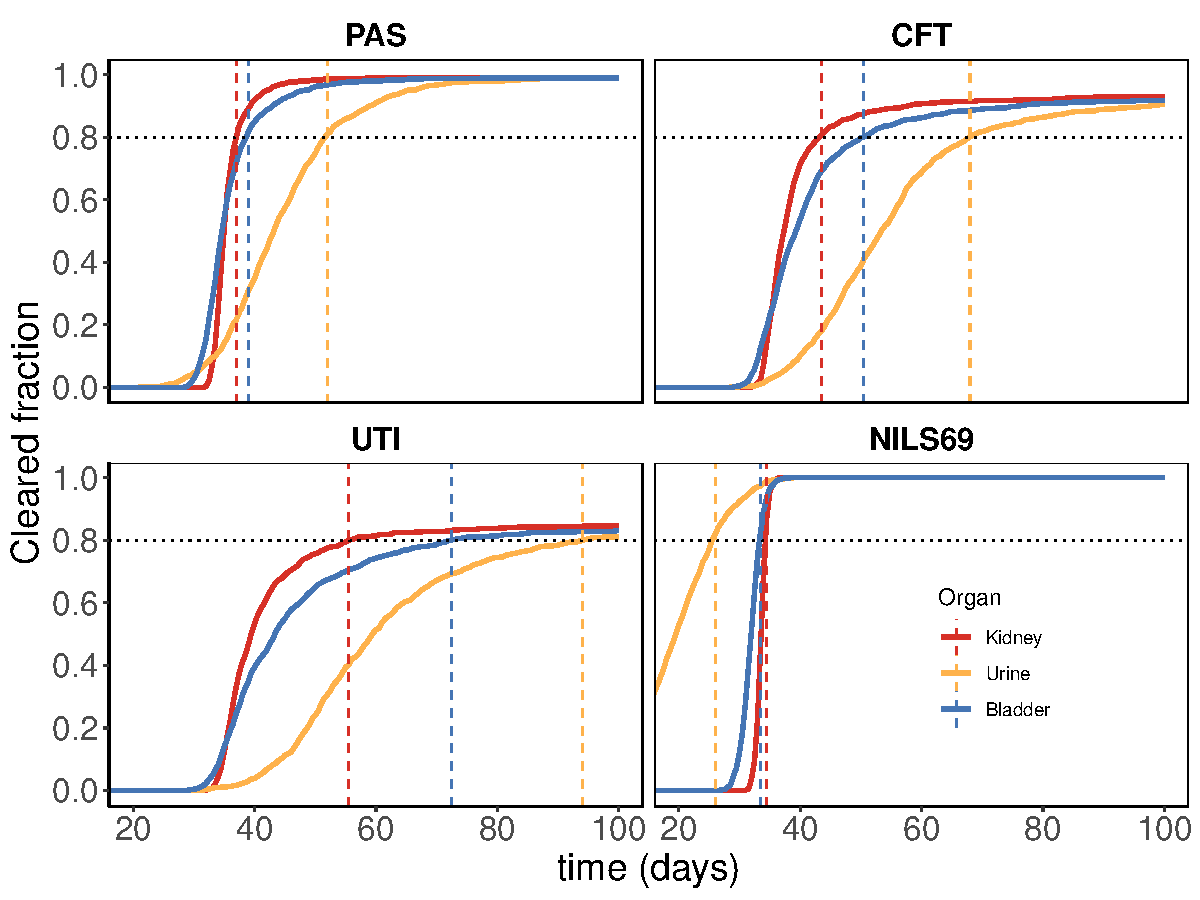
\includegraphics[width=\linewidth]{images/plt_final_model_Ct_strain_ALL_Clearence_Simul.pdf}
	\caption{Fraction of bacteria cleared over time by strain for each organ, based on results from 1,000 simulated mice per strain. The figure includes four panels, each corresponding to a different bacterial strain (PAS, CFT, UTI, and NILS69). The dotted horizontal line indicates the 80\% clearance threshold, and dashed vertical lines mark the specific time points at which each organ individually reaches this threshold}
	\label{fig:SimulationsClearedStrainsALL}
\end{figure}


%plt_final_model_Ct_strain_ALL_Clearence_Simul.pdf


\subsubsection{Model with antibiotic PAS strain}
%\TODO{directly in text, comments with RSE. }

We investigated the effect of the antibiotic on mice infected with the PAS strain, focusing on groups that received no treatment as well as those treated with two doses: 2.5 mg/kg and 10 mg/kg of ciprofloxacin.

The best model we could found for the antibiotic treatment was the linear effect Eq. \ref{eq:modelABLinear} acting on the $delta_{U}$ and $delta_{K}$ as 

\begin{alignat}{1}
\delta_{K}^{Cipro} &= \left(1 - \epsilon_K D^{Cipro} \right) \delta_{K} \nonumber \\
\delta_{U}^{Cipro} &= \left(1 + \epsilon_U D^{Cipro} \right) \delta_{U}
\end{alignat}




\begin{table}
	\begin{tabular}{|l|l|l|l|}
		\hline
		Parameter & Estimates(r.s.e.) & Units\\ \hline
		$\epsilon_{K}$ & $0.0057(17.4\%)$ & $g/(days.kg)$\\
		$\epsilon_{U}$ & $464.37(30.8\%)$ & $g/(days.kg)$\\
		\hline
	\end{tabular}
	\caption{Parameter estimates for model with antibiotic treatment.}
\end{table}




\section{Discussions}
\begin{itemize}
	\item Only one point per mice, is this consider longitudinal data?
\end{itemize}

\section{Conclusions}

\TODO{Fix it}
The competition of bacteria elimination and proliferation are different in the three compartments.
The relationship among bladder, kidney and urine exchange rates indicates that the urine compartment is the main path to elimination and the large proliferation in the kidney positions it as the primary source of a long lasting bacteria. The persistence of bacteria in the bladder despite the administration of ciprofloxacin, even at higher concentrations has been reported before.\cite{jakobsen2020ciprofloxacin} In this study we presented a reduced comprehensive mathematical model of the colonisation in UTI organs for PAS E. coli under the administration of two doses of ciprofloxacin which is the starting point to develop better models with other antibiotics with different mechanism of action and different strains.

Tab. \ref{tab:mice_sampling}

\section{Bibliography}
% \printbibliography %[heading=none,title=none]
\printbibliography % Print bibliography
% \bibliographystyle{plain} % We choose the "plain" reference style
% \bibliography{anoruti_refs} % Entries are in the refs.bib file

\appendix
\section{Data}
\TODO{Table Supp.}
\begin{table}[h!]
	\centering
	% Adjust the table size if needed
	\begin{adjustbox}{max width=\textwidth}
%		\begin{tabular}{|c|c|c|c|c|c|c|c|c|c|c|}
		\begin{tabular}{|p{3.5cm}|c|c|c|c|c|c|c|c|c|c|}
			\hline
			\makecell[c]{Antibiotic Group} & \makecell[c]{Strain} & \multicolumn{8}{c|}{Days} & \makecell[c]{Total} \\ \cline{3-10} 
			&                      & 1 & 2 & 4 & 6 & 10 & 14 & 16 & 22 & \\ \hline
			\multirow{4}{*}{Control} & PAS & 13 & 17 & 18 & 5 & 3 &  & 9 & 11 & 76 \\ \cline{2-11}
			& NILS69 &  & 15 & 12 &  &  &  &  &  & 27 \\ \cline{2-11}
			& UTI &  & 12 & 11 &  & 3 &  & 5 &  & 31 \\ \cline{2-11}
			& CFT &  & 11 & 13 &  & 8 &  & 8 &  & 40 \\ \hline
			\multirow{3}{*}{\makecell[c]{Ciprofloxacin 2.5 mg/kg }} % \\ 9 a.m and 5 p.m. \\for 48 hours.
			& PAS &  &  & 17 &  & 5 &  &  &  & 22 \\ \cline{2-11}
			& UTI &  &  & 7 &  &  &  &  &  & 7 \\ \cline{2-11}
			& CFT &  &  & 11 &  &  &  &  &  & 11 \\ \hline
			\multirow{4}{*}{\makecell[c]{Ciprofloxacin 10 mg/kg }} % 9 a.m and 5 p.m. \\for 48 hours.
			& PAS &  &  & 7 &  &  &  &  &  & 7 \\ \cline{2-11}
			& NILS69 &  &  & 7 &  &  &  &  &  & 7 \\ \cline{2-11}
			& UTI &  &  & 7 &  &  &  &  &  & 7 \\ \cline{2-11}
			& CFT &  &  & 6 &  &  &  &  &  & 6 \\ \hline
			\multirow{1}{*}{\makecell[c]{Cefotaxime 100 mg/kg}}  % \\ every 6 hours \\for 24 hours.
			& PAS &  &  & 14 &  & 6 &  &  &  & 20 \\ \hline
			\multirow{1}{*}{\makecell[c]{Fosfomycin 100 mg/kg }} % \\ every 4 hours \\for 24 hours.
			& PAS &  &  & 8 &  &  &  &  &  & 8 \\ \hline
			\multirow{1}{*}{\makecell[c]{Delafloxacin 10 mg/kg }} % \\ 9 a.m and 5 p.m. \\for 48 hours.
			& PAS &  &  & 7 &  &  &  &  &  & 7 \\ \hline
			& & 13 & 55 & 145 & 5 & 14 & 11 & 22 & 11 & 276 \\ \hline
		\end{tabular}
	\end{adjustbox}
	\caption{Mice sampling distribution with antibiotic treatments on bacterial strains in time.}
	\label{tab:mice_sampling}
\end{table}

\begin{figure}
	\centering
	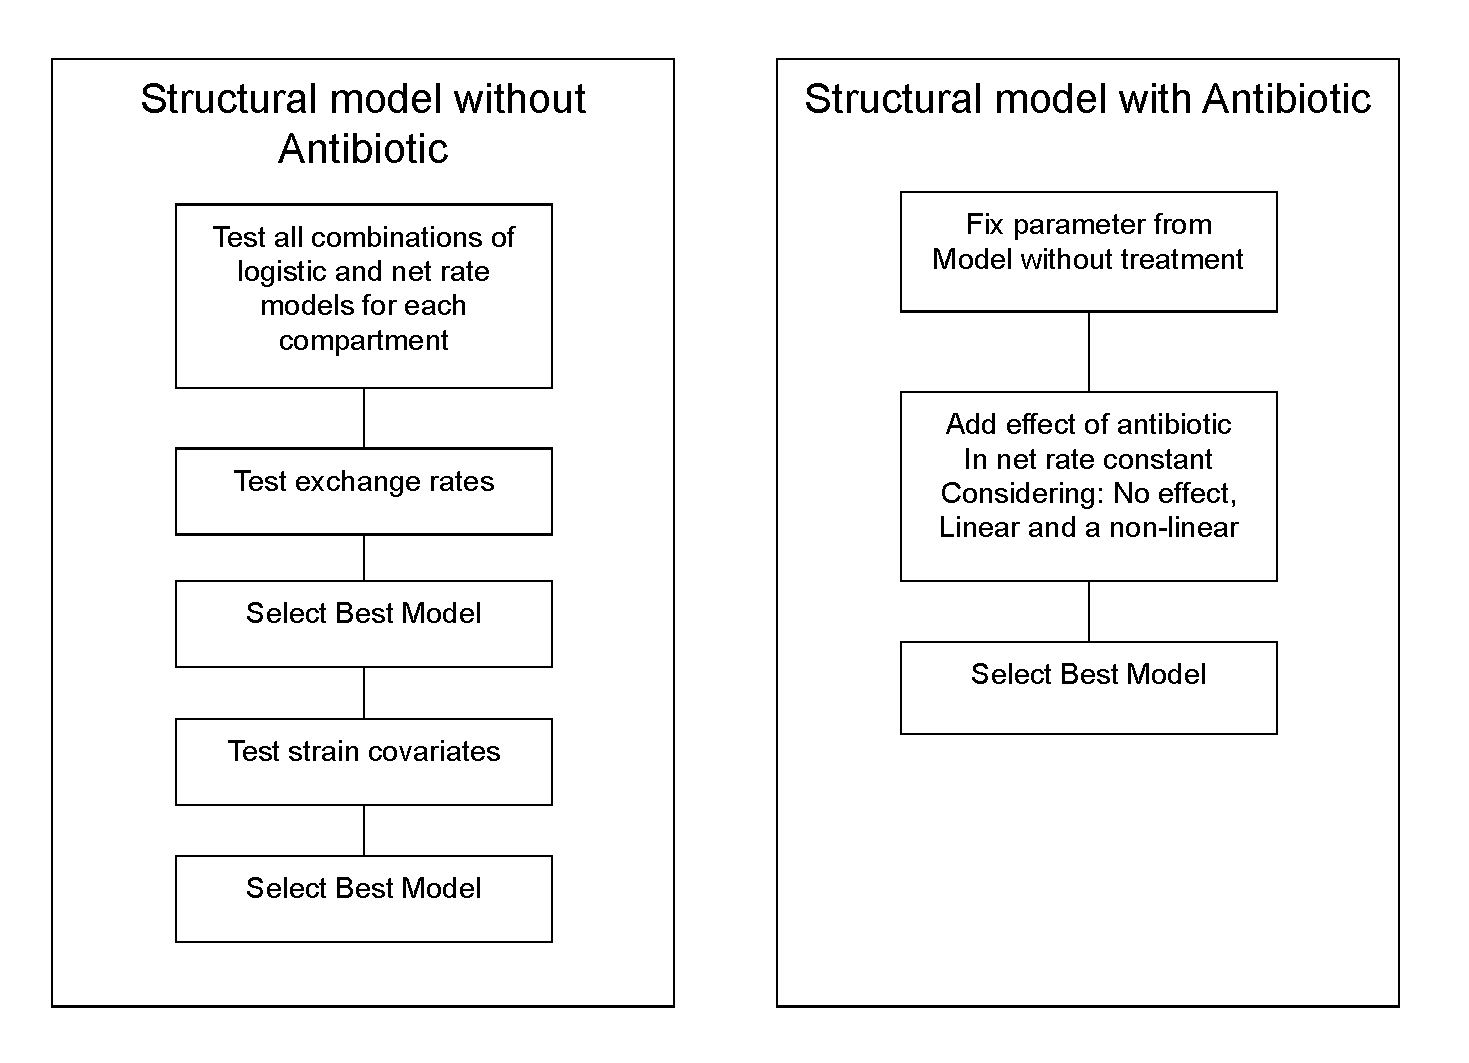
\includegraphics[width=0.8\linewidth]{images/anoruti_model_strategy_v002.pdf}
	\caption{Model diagram for PAS strain without antibiotic treatment. }
	\label{fig:ModelingStrategy}
\end{figure}


\begin{figure}
	\centering
	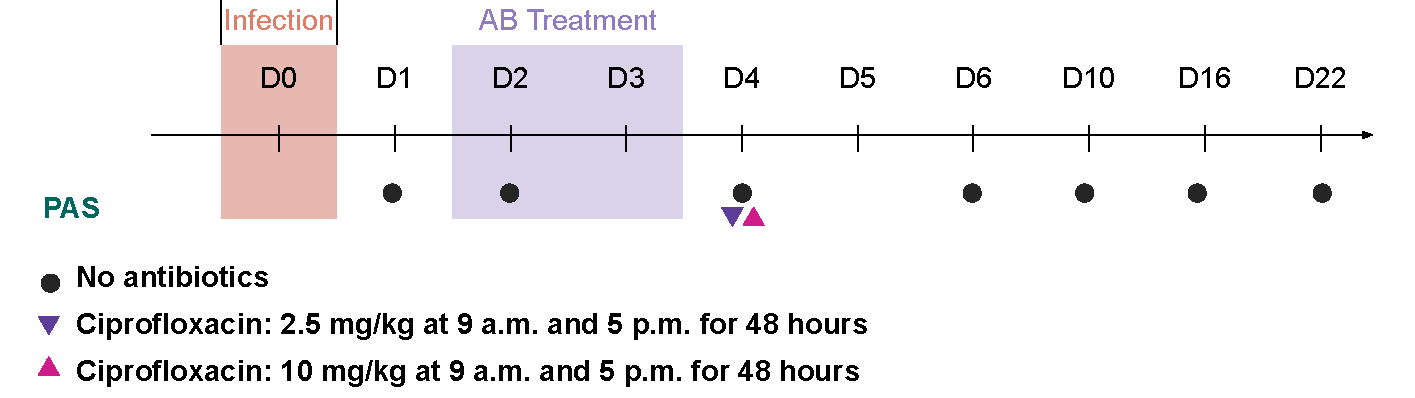
\includegraphics[width=0.8\linewidth]{images/draw_Anoruti_flowchart_PAS.pdf}
	\caption{Data description. }
	%		\label{fig:ModelOneline}
\end{figure}



%plt_vpc_merged_Ct_ONLY.pdf
\begin{figure}
	\centering
	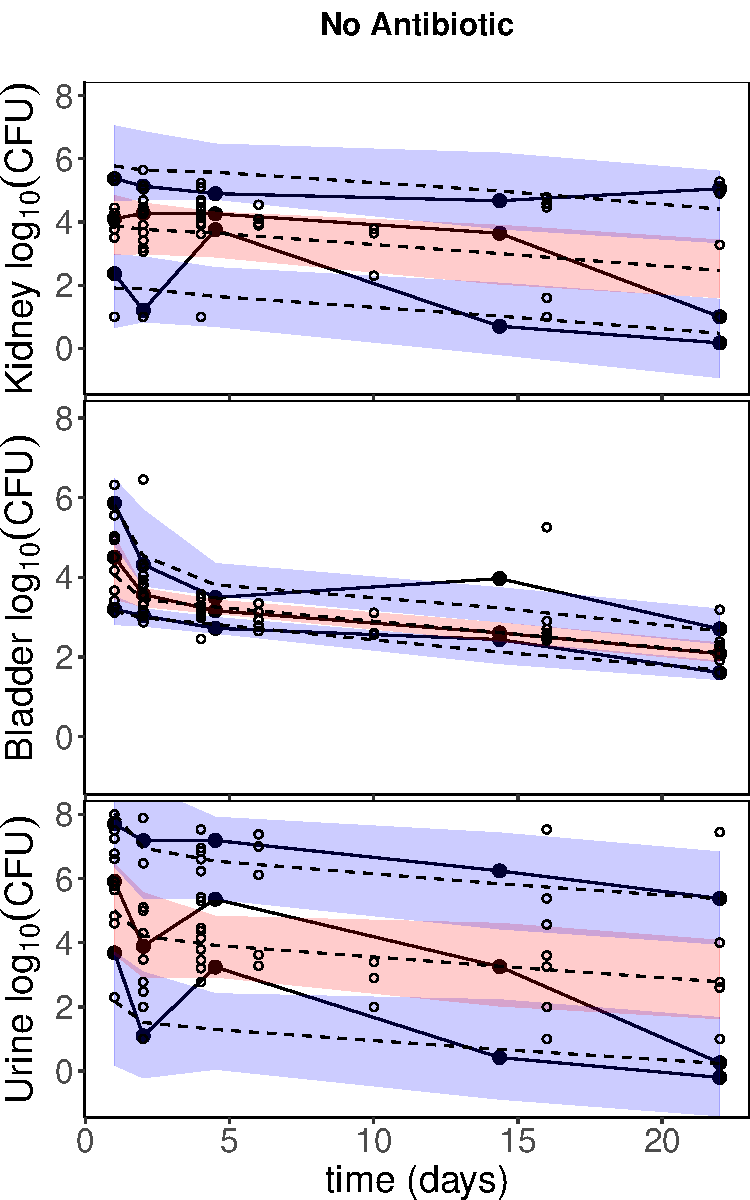
\includegraphics[width=\linewidth]{images/plt_vpc_merged_Ct_ONLY.pdf}
	\caption{Visual Predicte Check for model with antibiotic, for each compartment.}
	\label{fig:ModelIndFits}
\end{figure}



%final_model_Ct_PAS
\begin{figure}
	\centering
	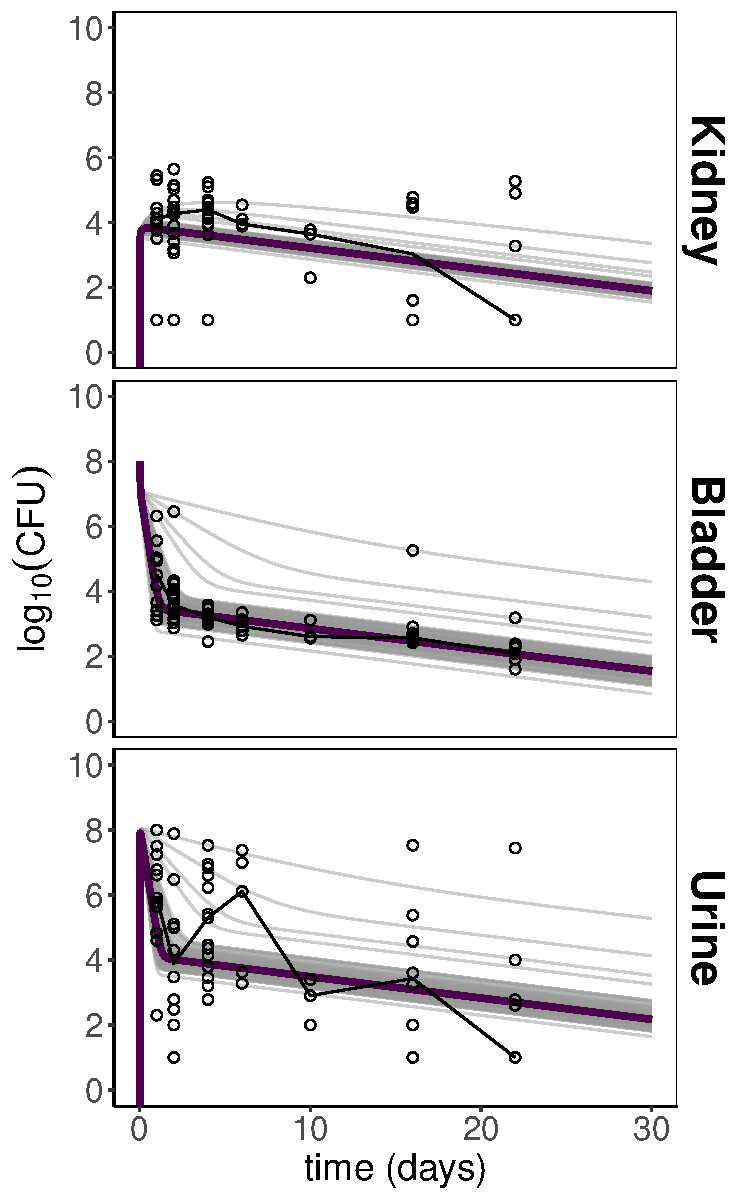
\includegraphics[width=\linewidth]{images/plt_final_model_Ct_PAS_vertical.pdf}
	\caption{Time evolution of CFU for each organ compartment, open circles experimental data, individual fits gray line, purple curve population parameters, black solid line medianvalue at each sampling day}
	\label{fig:ModelIndFits}
\end{figure}

\TODO{Change or remove sampling figure, maybe better to add numbers with the symbols or just text description.}

\begin{itemize}
	\item \TODO{Add table with mice organ distribution CFU counts? or write directly med [min;max]}
	\item \TODO{LacZ too? Let's see that later}
\end{itemize}


\subsection{Model evaluation}
\TODO{VPC, residuals?}




\begin{figure}
	\centering
	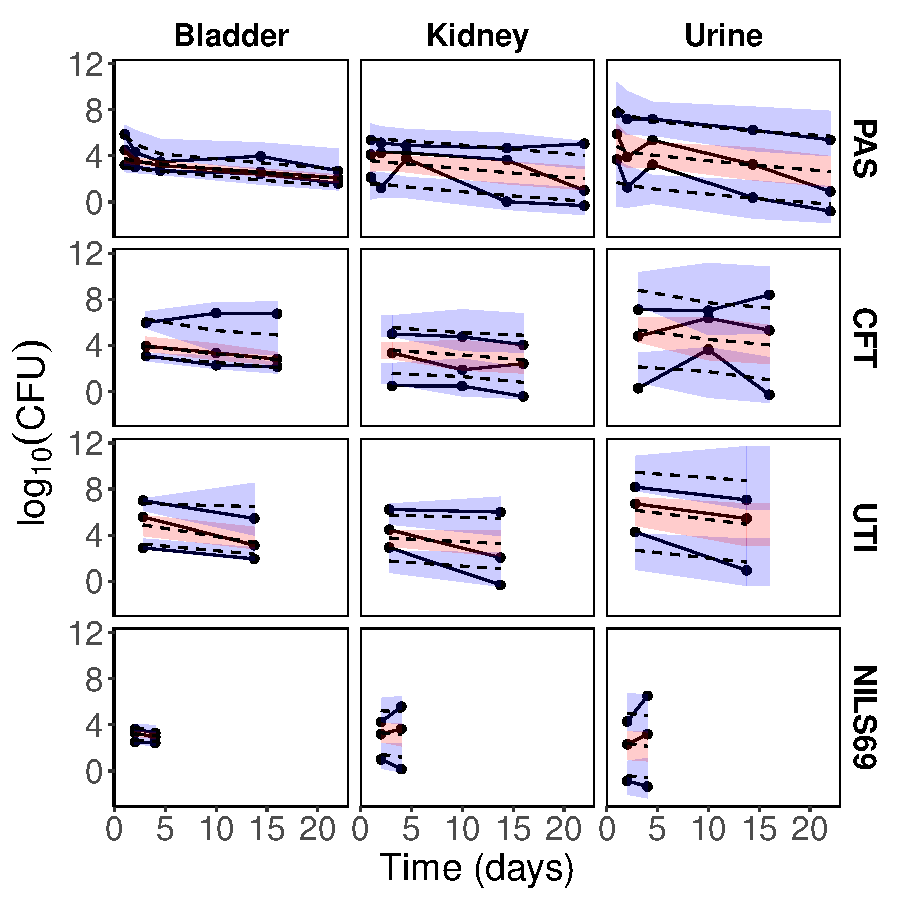
\includegraphics[width=\linewidth]{images/plt_final_model_Ct_ALL_VPC.pdf}
	\caption{Visual Predicte Check for different strains and compartments.}
	\label{fig:ModelIndFits}
\end{figure}




\subsubsection{Ethics Statement} 
\TODO{The study was conducted in accordance with the ethical standards of ... and received approval from the ... }


\TODO{Define order strain or antibiotic effect first? I think is better strain, because antibiotic has less data perhaps?}
\TODO{Make a better figure \ref{fig:ModelingStrategy} and include the strains}



\TODO{Should I include the logistic growth equations? I imaging that for completeness I could write it but maybe in the appendix. Or maybe a general equation for one compartment but probably will not be easy to read.}



\section{For Slides}

\begin{alignat}{2}
\delta_{K}^{AB} = \delta_{K}(1 - \mathbb{I}_{c,2} \epsilon_{K2} )
\end{alignat}

\begin{alignat}{2}
\frac{d}{dt} K &=  \delta_K^{AB}K &- q_{K,B} K + q_{B,K} B \\
\frac{d}{dt} B &=  \delta_B B &- q_{B,K} B + q_{K,B} K \nonumber\\
&              & -q_{B,U} B + q_{U,B} U \\
\frac{d}{dt} U &=  \delta_U U &- q_{U,B} U + q_{B,U} B
\end{alignat}


\begin{table}
	\begin{tabular}{|c|r|}
		\hline
		Parameter & Value [r.s.e.]\\
		& ($days^{-1}$)  \\ \hline
		$\delta_{K}$ & $8.4$ [2\%]\\
		$\delta_{B}$ & $18.7$ [NA\%] \\
		$\delta_{U}$ & $-6.7$ [NA\%] \\
		$q_{BK}$ & $0.002$ [NA\%] \\
		$q_{KB}$ & $8.6$ [2\%] \\
		$q_{BU}$ & $38$ [16\%] \\
		$q_{UB}$ & $0.42$ [7\%] \\
		\hline
	\end{tabular}
	%	\label{tab:FinalModelPAS}
	\caption{No variability.}
\end{table}


2
\begin{table}
	\begin{tabular}{|c|r|}
		\hline
		Parameter & Value [r.s.e.]\\ 
		 & ($days^{-1}$)\\ \hline
		$\delta_{K}$ & $8.8$ [NA] \\
		$\delta_{B}$ & $20.1$ [11\%]\\
		$\delta_{U}$ & $-7.4$ [11\%]\\
		$q_{BK}$ & $0.002$ [60\%] \\
		$q_{KB}$ & $8,9$ [1\%] \\
		$q_{BU}$ & $59$ [16\%] \\
		$q_{UB}$ & $1.7$ [2\%] \\ \hline
		$\omega_{\delta_{U}}$ & $2.9$ [20\%]\\
		\hline
	\end{tabular}
	%	\label{tab:FinalModelPAS}
	\caption{Varibility in 1 parameter}
\end{table}




\begin{table}
	\begin{tabular}{|c|r|}
		\hline
		Parameter & Value[r.s.e.]\\ 
		 & ($days^{-1}$) \\ \hline
%		 & [r.s.e.] & ($\%$)\\ \hline
		$\delta_{K}$ & $12.2$ [1\%] \\
		$\delta_{B}$ & $12.7$ [11\%] \\
		$\delta_{U}$ & $-9.8$ [31\%] \\
		$q_{BK}$ & $0.002$ [92\%] \\
		$q_{KB}$ & $12$ [1\%] \\
		$q_{BU}$ & $59$ [36\%] \\
		$q_{UB}$ & $4.2$ [17\%] \\ \hline
		$\omega_{\delta_{U}}$ & $3.4$ [40\%]\\
		$\omega_{q_{BU}}$ & $0.23$ [25\%]\\
		\hline
	\end{tabular}
%	\label{tab:FinalModelPAS}
	\caption{Final model only PAS}
\end{table}


4

\begin{align}
	\delta_{U}^{PAS} &= \delta_{U} \\
	\delta_{U}^{CFT} &= \delta_{U} + \beta_{\delta_{U}, CFT} \\
	\delta_{U}^{UTI} &= \delta_{U} + \beta_{\delta_{U}, UTI} \\
	\delta_{U}^{NILS69} &= \delta_{U} + \beta_{\delta_{U}, NILS69} \\
\end{align}

\begin{table}
	\begin{tabular}{|c|r|}
		\hline
		Parameter & Value[r.s.e.] \\ 
		 & ($days^{-1}$) \\ \hline
		$\delta_{K}$ & $40[0.74\%]$ \\
		$\delta_{B}$ & $13[19.26\%]$ \\
		$\delta_{U}$ & $-12[33.15\%]$ \\
		$q_{BK}$ & $ 0.0016[34.95\%]$ \\
		$q_{KB}$ & $40[0.74\%]$ \\
		$q_{BU}$ & $66[10.84\%]$ \\
		$q_{UB}$ & $2[6.86\%]$ \\ \hline
		$\omega_{\delta_{U}}$ & $1.2[15.28\%]$ \\
		$\omega_{q_{BU}}$ & $0.11[40.13\%]$ \\
		\hline
		$\beta_{\delta_{U}, CFT}$ & $1.1 [30.03\%]$ \\
		$\beta_{\delta_{U}, UTI}$ & $1.6 [23.54\%]$ \\
		$\beta_{\delta_{U}, NILS69}$ & $-3.8 [25.51\%]$ \\
		%		$\sigma$
		\hline
	\end{tabular}
	\caption{Final model estimates with all strains.}
\end{table}

\end{document}
